\documentclass[english]{beamer}
\usepackage[english]{babel}
\usepackage{bookmark}
\usepackage[utf8]{inputenx}
\usepackage[T1]{fontenc}      % Font encoding
\usepackage{lmodern}          % lmodern font, correctly copyable characters in pdf
\usepackage{microtype}
\usepackage{graphicx}
\usepackage{subcaption}
\usepackage{wasysym}
\usepackage{algpseudocode}
\usepackage{tabularx}

\usetheme[
  bullet=circle,                  % Use circles instead of squares for bullets
  titleline=false,                % Show a line below the frame
  alternativetitlepage=true,      % Use the fancy title
  titlepagelogo=logo-sapienza,    % Logo for the first slide
  watermark=watermark-diag,   % Watermark used in every slide
  watermarkheight=20px,           % Desired height of the watermark
  watermarkheightmult=6,          % Watermark image is actually x times bigger
  displayauthoronfooter=true,     % Display author name in the footer
]{Roma}
\watermarkoff
\author{Giuseppina Iannotti, 1938436\\Davide Marincione, 1927757}
\title{A multimodal interface for chess}
\subtitle{How we made people gesticulate and scream at their computers}
\institute{Sapienza, University of Rome}
\date{A. Y. 2023 - 2024}

\begin{document}

\begin{frame}[t, plain]
\titlepage
\end{frame}

\section{Introduction}
\begin{frame}[c]{The Idea}
    Remember this?
    \begin{figure}
        \centering
        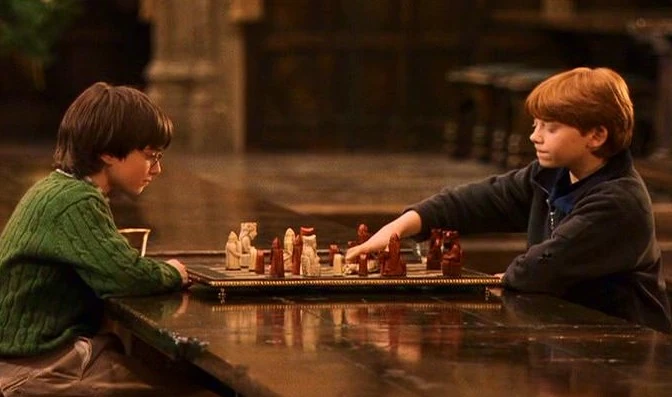
\includegraphics[width=.85\textwidth]{images/wizard_chess.png}
        \caption{Wizard's Chess, Harry Potter and the Philosopher's Stone}
    \end{figure}
\end{frame}

\begin{frame}[c]{The Idea 2}
    Know this feeling?
    \begin{figure}
        \centering
        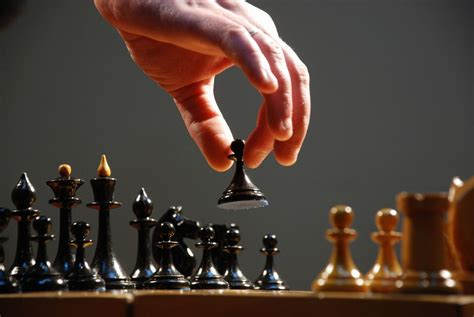
\includegraphics[width=.7\textwidth]{images/stock_hand.jpeg}
        \caption{Some stock image of an hand holding a chess piece.}
    \end{figure}
\end{frame}

\section{Code, Graphics, and Sound}
\begin{frame}{Before that}
    \begin{columns}[T]
        \begin{column}{.5\textwidth}
            We have to get from here\dots
            \begin{figure}
                \centering
                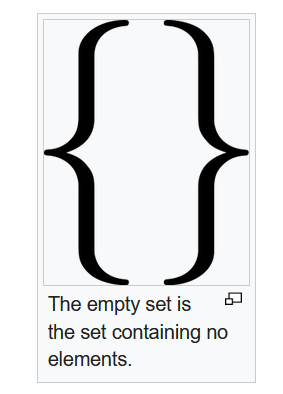
\includegraphics[width=.65\textwidth]{images/empty_set.png}
                \caption{What we have.}
            \end{figure}
        \end{column}
        \begin{column}{.5\textwidth}
            To here!
            \begin{figure}
                \centering
                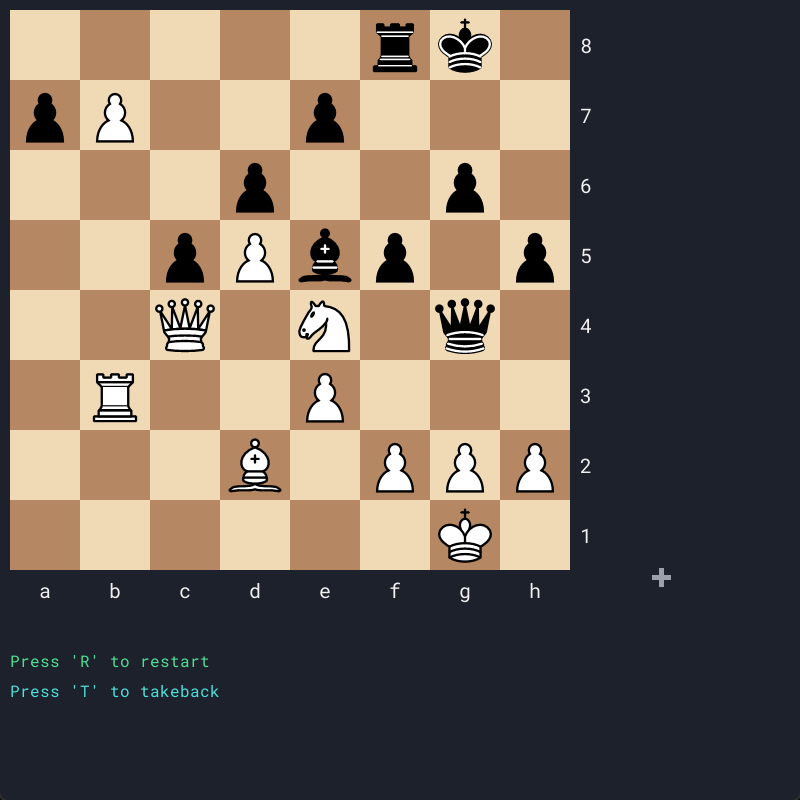
\includegraphics[width=.9\textwidth]{images/gui_example.png}
                \caption{What we want.}
            \end{figure}
        \end{column}
    \end{columns}
\end{frame}

\begin{frame}{We need some OOP}
    \begin{figure}
        \centering
        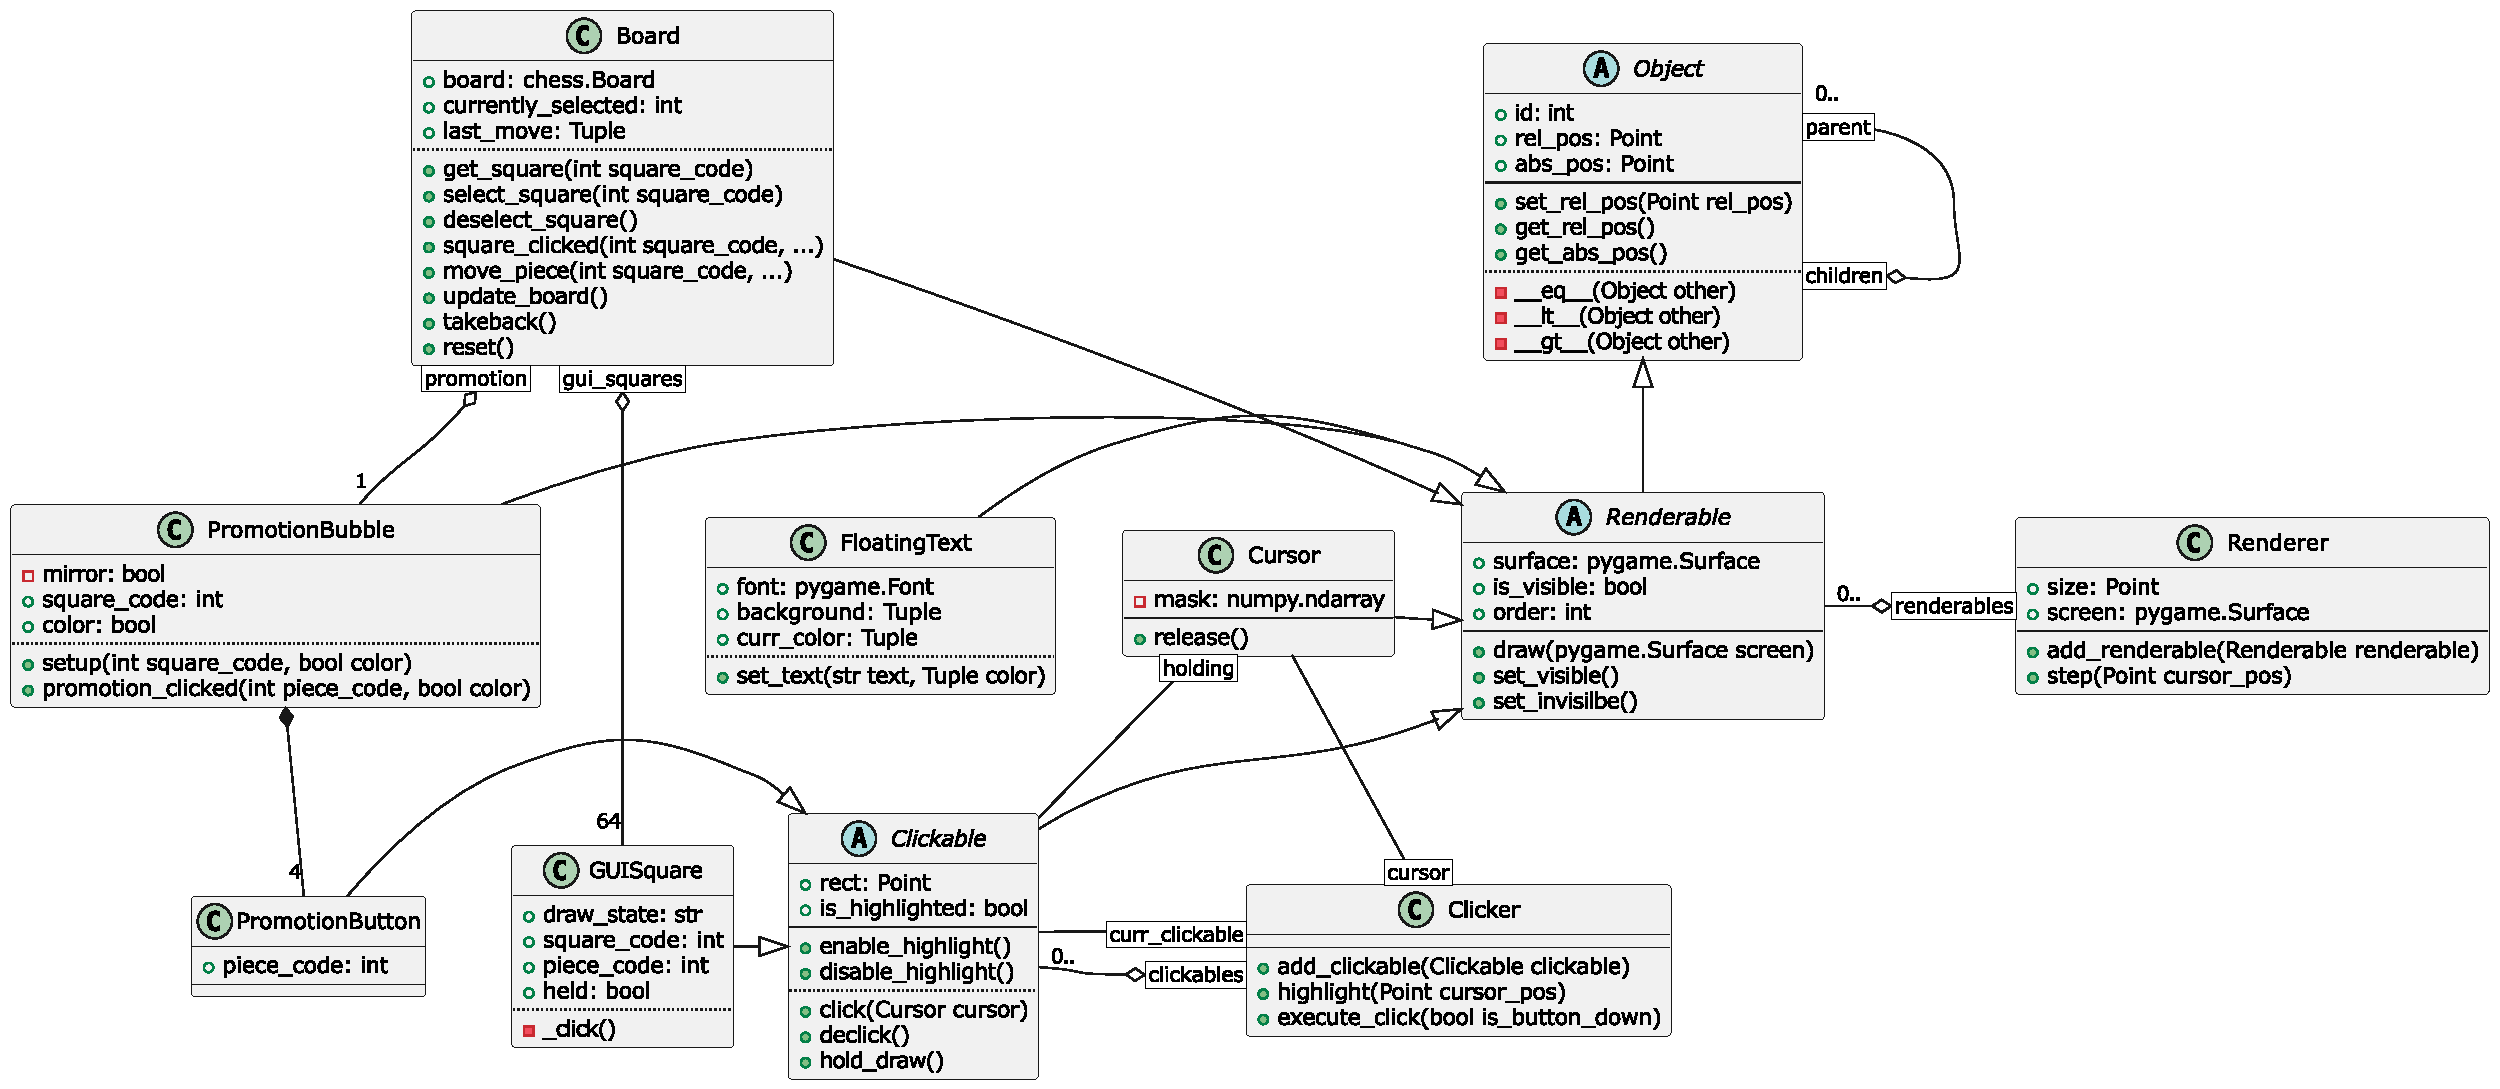
\includegraphics[width=.98\textwidth]{images/uml.pdf}
        \caption{Class diagram of the game's elements}
    \end{figure}
\end{frame}

\begin{frame}{A bit in detail 1}
    \begin{columns}[T]
        \begin{column}{.5\textwidth}
            The \texttt{Renderer}\dots draws \texttt{Renderables}!
            \begin{enumerate}
                \item Keeps track of them.
                \item Draws them based on each object's \texttt{order} attribute.
                \item Draws them only if they are set to visible.
            \end{enumerate}
        \end{column}
        \begin{column}{.5\textwidth}
            The \texttt{Clicker}:
            \begin{enumerate}
                \item Keeps track of the \texttt{Clickable}s.
                \item Highlights the current \texttt{Clickable}, calls its click/declick method.
                \item Drives hold/release with \texttt{Cursor}.
            \end{enumerate}
        \end{column}
    \end{columns}
\end{frame}

\begin{frame}{A bit in detail 2}
    \begin{columns}[T]
        \begin{column}{.5\textwidth}
            Our \texttt{Cursor} is this neat thing:
            \begin{figure}
                \centering
                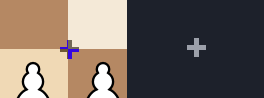
\includegraphics[width=.98\textwidth]{images/cursor_comparison.png}
                \caption{Our \texttt{Cursor}.}
            \end{figure}
        \end{column}
        \begin{column}{.5\textwidth}
            It is simple, but we are pretty happy about it:
            \begin{enumerate}
                \item It is extremely visible, because of the dynamic color
                \begin{equation*}
                    c^* = (c + 128)\ \mathrm{mod}\ 256.
                \end{equation*}
                \item It can hold pieces.
                \item Being stylistically different might have helped!
            \end{enumerate}
        \end{column}
    \end{columns}
\end{frame}

\begin{frame}{A bit in detail 3}
    \begin{columns}
        \begin{column}{.5\textwidth}
            The \texttt{Board}:
            \begin{enumerate}
                \item Wraps a \texttt{chess.Board} object (and all its complicated chess logic).
                \item Handles the state of all the \texttt{GUISquare} and that of the \texttt{PromotionBubble}.
                \item Plays audio when moves are done!
            \end{enumerate}
        \end{column}
        \begin{column}{.5\textwidth}
            \begin{figure}
                \centering
                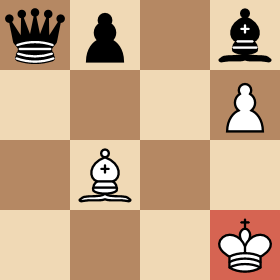
\includegraphics[width=.4\textwidth]{images/check_coloring.png}
                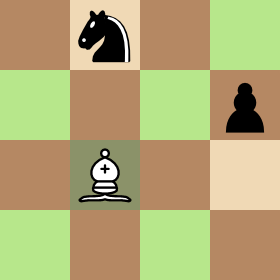
\includegraphics[width=.4\textwidth]{images/moves_coloring.png}
                \caption{Examples of \texttt{GUISquare} states}
                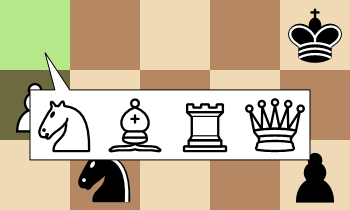
\includegraphics[width=.65\textwidth]{images/promotion_ex.png}
                \caption{What \texttt{PromotionBubble} looks like}
            \end{figure}
        \end{column}
    \end{columns}
\end{frame}

\begin{frame}{The main loop}
    All of this runs on the main thread, within the loop:

    \begin{enumerate}
        \item Update cursor with latest mouse or hand position.
        \item \texttt{clicker.highlight(cursor\_pos)}.
        \item Resolve events, such as mouse clicks, key presses (quit game, takebacks), and moves done (for the AI).
        \item Resolve voice commands.
        \item \texttt{renderer.step()}.
        \item Run metrics recorder.
    \end{enumerate}
\end{frame}


\section{Voice commands}

\begin{frame}{Dragonfly? What's that?}
    \begin{columns}[T]
        \begin{column}{.5\textwidth}
            Not this\dots
            \begin{figure}
                \centering
                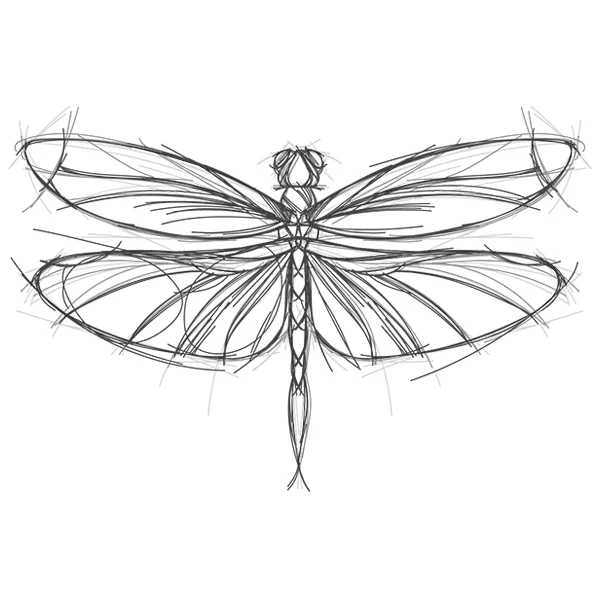
\includegraphics[height=.65\textwidth]{images/dragonfly.png}
                \caption{The insect.}
            \end{figure}
        \end{column}
        \begin{column}{.5\textwidth}
            This!
            \begin{figure}
                \centering
                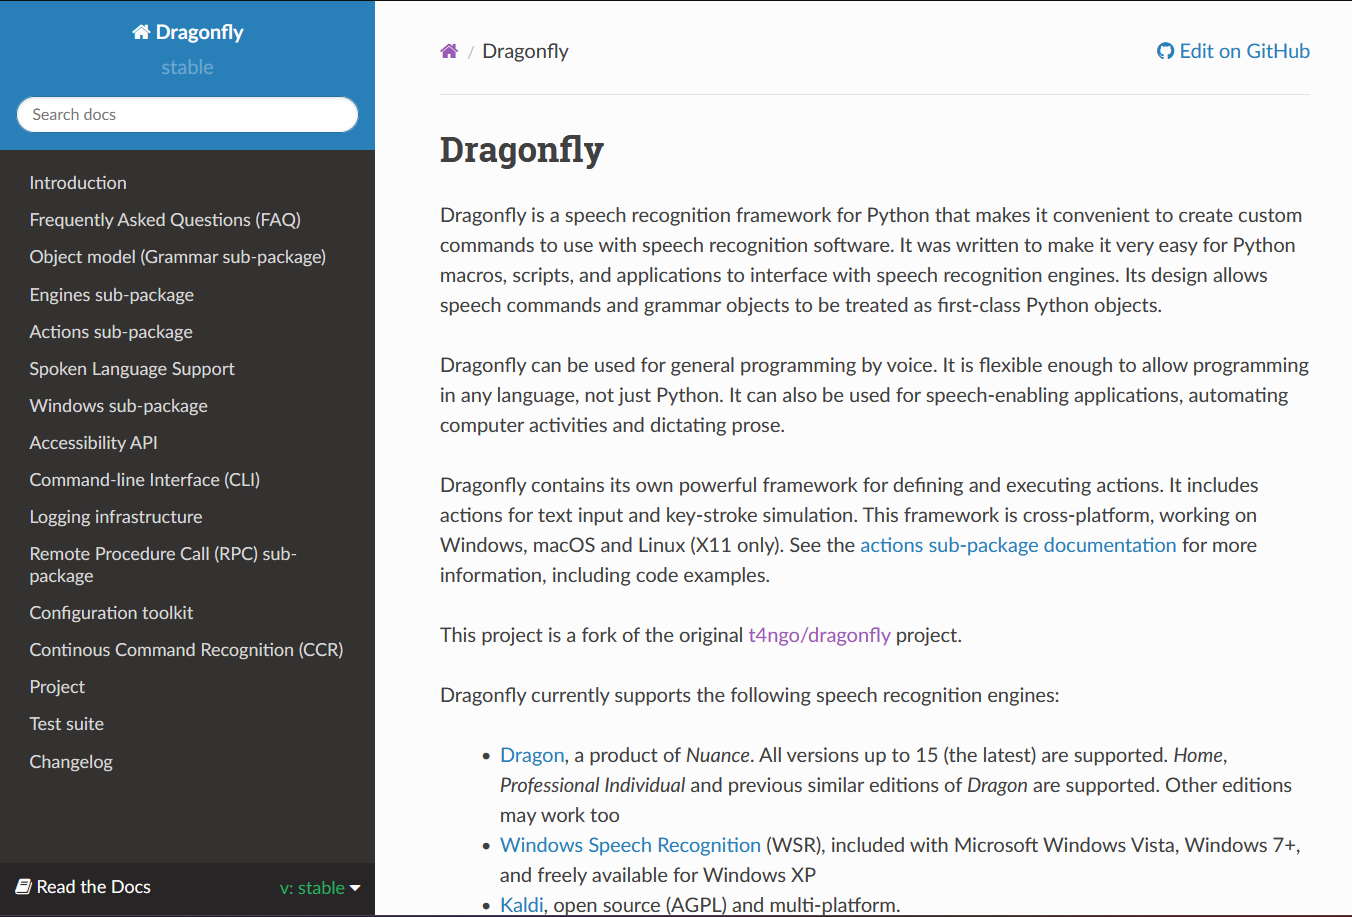
\includegraphics[height=.7\textwidth]{images/dragonfly_python.png}
                \caption{The package.}
            \end{figure}
        \end{column}
    \end{columns}
\end{frame}

\begin{frame}{Hey, but what is a Rule?}
    \begin{figure}
        \centering
        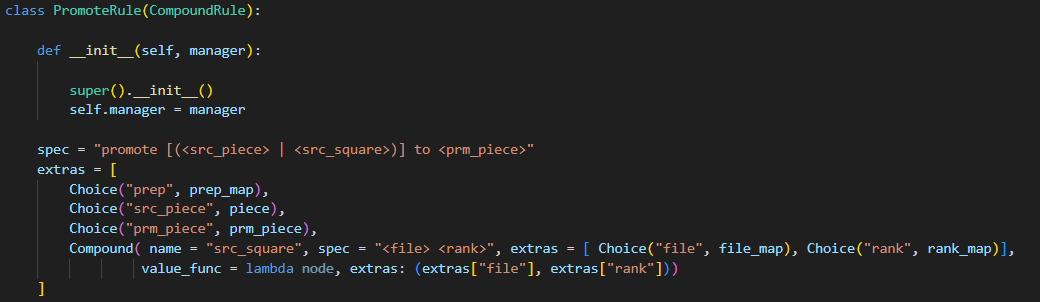
\includegraphics[width=\textwidth]{images/compound_rule.png}
        \caption{Example of Compound Rule}
    \end{figure}
    Each rule is instantiated as a \texttt{Compound Rule}, with parameters : 
    \begin{itemize}
        \item \texttt{spec} : Compound specification for the rules root element 
        \item \texttt{extras} :  Extras elements referenced from the compound spec, like choices for prepositions, pieces, and squares.
    \end{itemize}
\end{frame}

\begin{frame}{Hey, but what is a Rule? - ALTERNATIVE}
    % Simply this slide 
    Each rule is instantiated as a \texttt{Compound Rule}, with parameters : 
    \begin{itemize}
        \item \texttt{spec} : Compound specification for the rules root element 
        \item \texttt{extras} :  Extras elements referenced from the compound spec, like choices for prepositions, pieces, and squares.
    \end{itemize}
    It is characterized by a process recognition method that bla bla bla 
\end{frame}


\begin{frame}{Rules I}
    \begin{table}[h]
        \centering
        \caption{Rules I}
        \small % Adjust font size as needed
        \begin{tabularx}{1.0\textwidth}{|l|X|} % Adjust width here, e.g., 1.0\textwidth
            \hline
            \textbf{Rule Name} & \textbf{Specification} \\
            \hline
            Move Rule & \texttt{"move ( [ <src\_piece>] | [ <src\_piece> [<prep> <src\_square>] to <tgt\_square>] | [ [<prep>] <src\_square> to <tgt\_square>]) [and promote to <prm\_piece>]"} \\
            \hline
            Capture Rule & \texttt{"capture (<tgt\_piece> [<prep> <tgt\_square>] | <tgt\_square>) [with (<src\_piece> [<prep> <src\_square>] | <src\_square>)] [and promote to <prm\_piece>]"}\\
            \hline
            Promote Rule & \texttt{"promote [(<src\_piece> | <src\_square>)] to <prm\_piece>"} \\
            \hline 
        \end{tabularx}
        \label{tab:rules}
    \end{table}
\end{frame}


\begin{frame}{Rules 2}
    \begin{table}[h]
        \centering
        \caption{Rules II}
        \small % Adjust font size as needed
        \begin{tabularx}{1.0\textwidth}{|l|X|} % Adjust width here, e.g., 1.0\textwidth
            \hline
            \textbf{Rule Name} & \textbf{Specification} \\
            \hline 
            Castle Rule & \texttt{"(castle <special\_direction> | <special\_direction> castle)"} \\
            \hline 
            Piece Rule & \texttt{"<src\_piece> ( [<prep>] <tgt\_square> |in <src\_square> <verb> [<prep>] ( <tgt\_square> | <tgt\_piece> [in <tgt\_square>] ) | <verb> [<prep> <src\_square>]( [<prep>] <tgt\_square> | <tgt\_piece>  [in <tgt\_square>])) [and promote to <prm\_piece>]"}\\
            \hline
            Square Rule & \texttt{"<src\_square> <verb> ( [<prep>] <tgt\_square> | <tgt\_piece> [<prep> <tgt\_square>])"}\\
            \hline
        \end{tabularx}
        \label{tab:rules}
    \end{table}
\end{frame}

\begin{frame}{Validating commands}
\end{frame}


\section{Hand tracking \& gestures}
\begin{frame}{Good ol' mediapipe}
    \begin{columns}
        \begin{column}{.5\textwidth}
            Of course, we use \texttt{mediapipe} for hand tracking.
            \begin{figure}
                \centering
                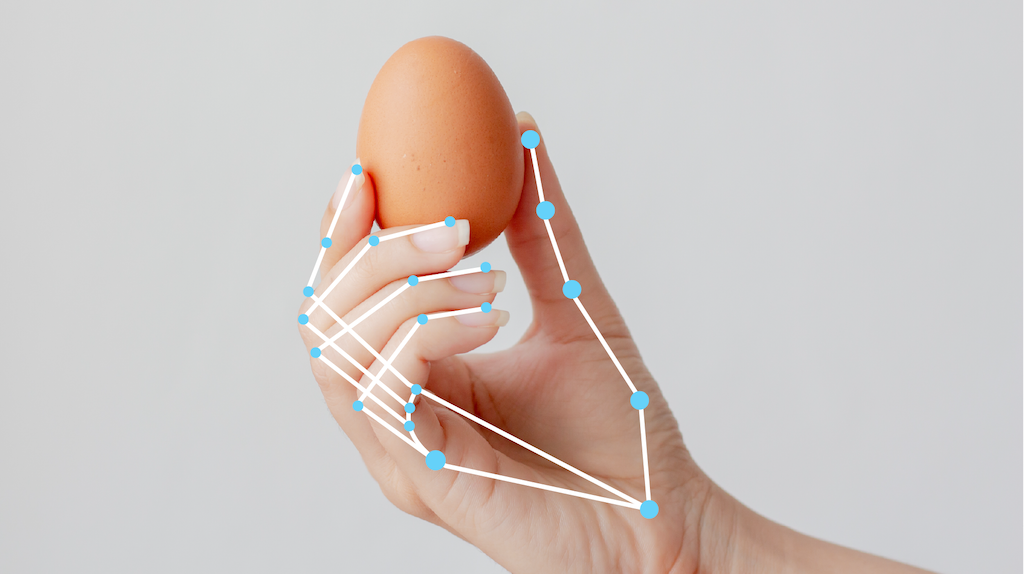
\includegraphics[width=.9\textwidth]{images/hand_landmark.png}
                \caption{You know what this is.}
            \end{figure}
        \end{column}
        \begin{column}{.5\textwidth}
            \begin{enumerate}
                \item We run it on a separate thread (\texttt{HandDetector}).
                \item Process it for our needs.
                \item Make it temporally coherent.
            \end{enumerate}
        \end{column}
    \end{columns}
\end{frame}

\begin{frame}{'Hand'made normalization 1}
    Get palm center:
    \begin{equation}
        p = \frac{\mathbf{L}_1}{2} + \frac{\mathbf{L}_6 + \mathbf{L}_{10} + \mathbf{L}_{14} + \mathbf{L}_{18}}{8}.
    \end{equation}
    Its width
    \begin{equation}
        w = ||\mathbf{L}_6 - \mathbf{L}_{18}||_2,
    \end{equation}
    and compute the relative position:
    \begin{equation}
        \overline{\mathbf{L}} = \frac{\mathbf{L} - p}{w}.
    \end{equation}
\end{frame}

\begin{frame}{'Hand'made normalization 2}
    Find the palm's normal:
    \begin{equation}
        \mathbf{n}_{\mathrm{palm}} = (1 - \mathbf{2}_{\textrm{left}})\frac{(\mathbf{L}_6 - \mathbf{L}_1)\times(\mathbf{L}_{18} - \mathbf{L}_1)}{||(\mathbf{L}_6 - \mathbf{L}_1)\times(\mathbf{L}_{18} - \mathbf{L}_1)||_2}.
    \end{equation}
    Then we get the pinky normal,
    \begin{equation}
        \mathbf{n}_{\mathrm{pinky}} = (1 - \mathbf{2}_{\textrm{left}})\frac{\mathbf{n}_{\mathrm{palm}}\times(\mathbf{L}_{10} - \mathbf{L}_1)}{||\mathbf{n}_{\mathrm{palm}}\times(\mathbf{L}_{10} - \mathbf{L}_1)||_2}.
    \end{equation}
    And the fingers' normal,
    \begin{equation}
        \mathbf{n}_{\mathrm{fingers}} = (1 - \mathbf{2}_{\textrm{left}})\frac{\mathbf{n}_{\mathrm{pinky}}\times \mathbf{n}_{\mathrm{palm}}}{||\mathbf{n}_{\mathrm{pinky}}\times \mathbf{n}_{\mathrm{palm}}||_2}.
    \end{equation}
\end{frame}

\begin{frame}{'Hand'made normalization 3}
    Finally, 
    \begin{equation}
        \mathbf{L}^\star = \overline{\mathbf{L}}\left[\mathbf{n}_{\mathrm{pinky}}, \mathbf{n}_{\mathrm{fingers}}, \mathbf{n}_{\mathrm{palm}}\right]^T
    \end{equation}
    \begin{figure}
        \centering
        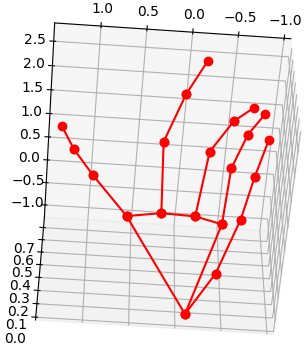
\includegraphics[width=.4\textwidth]{images/norm_hand.png}
        \caption{A right hand, normalized}
    \end{figure}
\end{frame}

\begin{frame}{Gesture recognition}
    \begin{columns}
        \begin{column}{.3\textwidth}
            At first, we wanted two gestures:
            \begin{enumerate}
                \item Tapping gesture, for "clicks". \frownie{}
                \item Grabbing gesture, to hold pieces. \smiley{}
            \end{enumerate}
        \end{column}
        \begin{column}{.7\textwidth}
            \begin{figure}
                \centering
                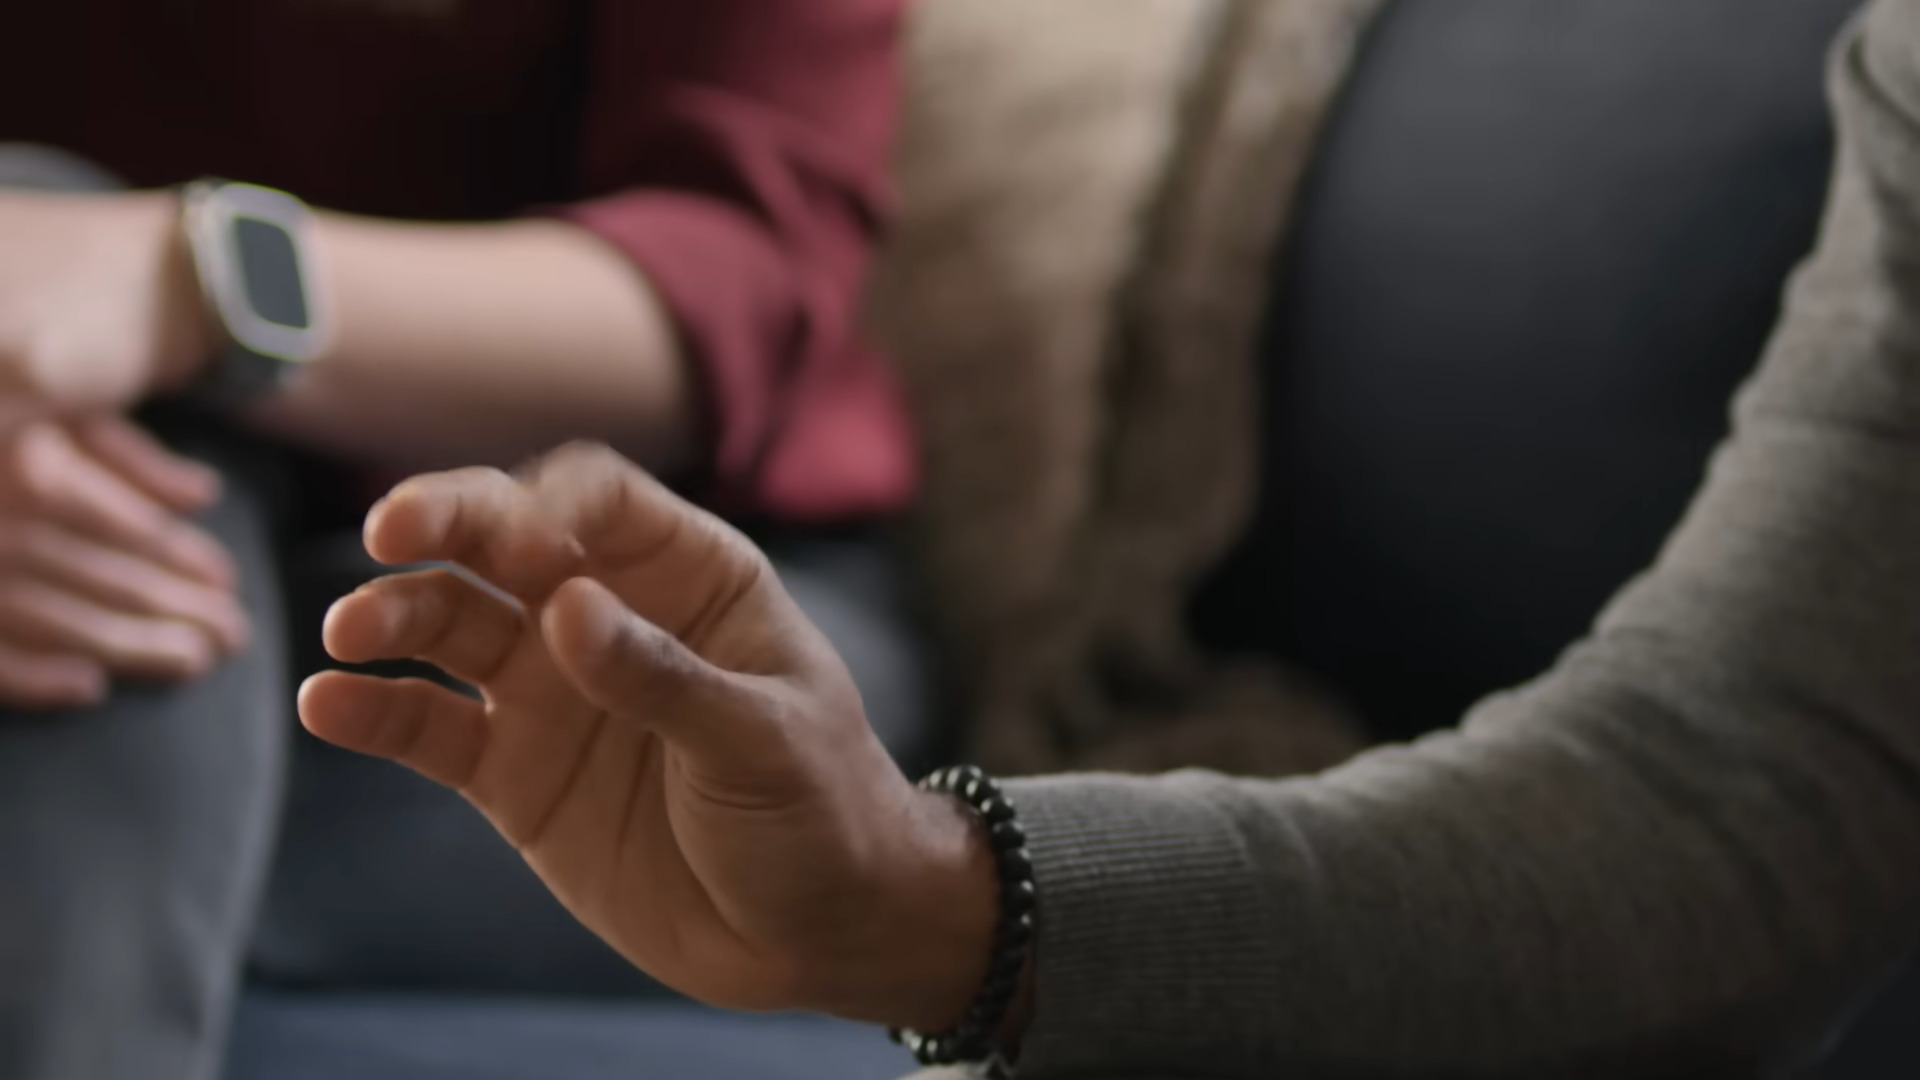
\includegraphics[width=.9\textwidth]{images/apple_click.jpg}
                \caption{Frame from "A Guided Tour of Apple Vision Pro"}
            \end{figure}
        \end{column}
    \end{columns}
\end{frame}

\begin{frame}{Recognizing grab}
    \begin{columns}
        \begin{column}{.5\textwidth}
            Very simple: hysteresis.

            \begin{algorithmic}[1]
                \State \textbf{input} \texttt{prev\_click}
                \State $m \gets ||\mathbf{L}^\star_{\mathrm{thumb}} - \mathbf{L}^\star_{\mathrm{index}}||_2$
                \State $d \gets \frac{\mathbf{L}^\star_{\mathrm{thumb}}\cdot\mathbf{L}^\star_{\mathrm{index}}}{||\mathbf{L}^\star_{\mathrm{thumb}}||_2 ||\mathbf{L}^\star_{\mathrm{index}}||_2}$
                \If{\texttt{prev\_click}}
                    \State \textbf{return} $m < \alpha_\gamma \land d > \beta_\gamma$
                \Else
                    \State \textbf{return} $m < \alpha \land d > \beta$
                \EndIf
            \end{algorithmic}
        \end{column}
        \begin{column}{.5\textwidth}
            Remember the Canny edge detector?
            \begin{figure}
                \centering
                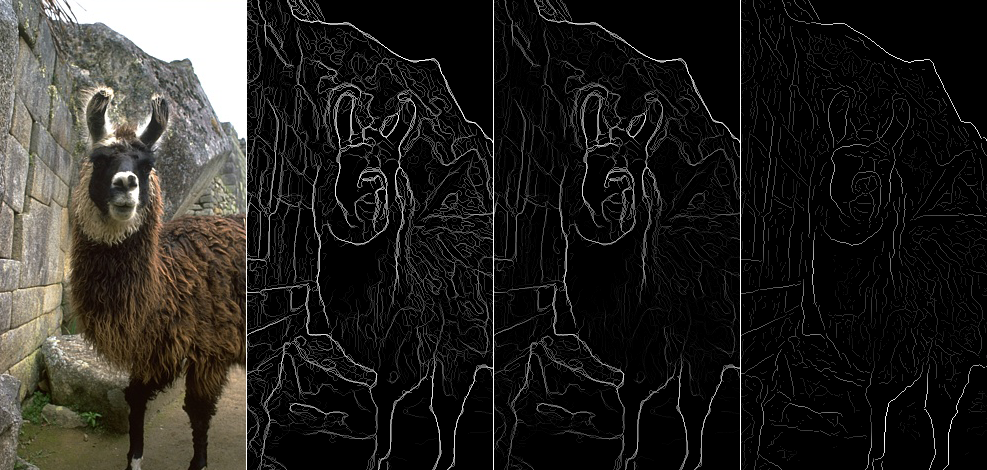
\includegraphics[width=\textwidth]{images/canny.png}
            \end{figure}
            That uses hysteresis too!
        \end{column}
    \end{columns}
\end{frame}

\begin{frame}{Hand2Cursor mapping}
    \begin{columns}
        \begin{column}{.5\textwidth}
            The direct mapping is
            \begin{equation}
                r = \mathrm{clip}_{[m,M]}(\frac{p - m}{M - m}).
            \end{equation}
            But we can't directly use $r$\dots\\
            Let $c$ be the internal cursor of \texttt{HandDetector}.
        \end{column}
        \begin{column}{.5\textwidth}
            \begin{enumerate}
                \item Noisy tracking: $c$ moves at constant rate, either bilinear or linear interpolation, if $r_{t-1}$ present.
                \item Cursor moving when hand still: only update if distance is enough.
                \item Random dropping of pieces: keep a list of most recent detections, if even one is a grab then output a grab.
            \end{enumerate}
        \end{column}
    \end{columns}
\end{frame}


\section{Experiments}
\begin{frame}{Recording System I}
    \begin{figure}
        \centering
        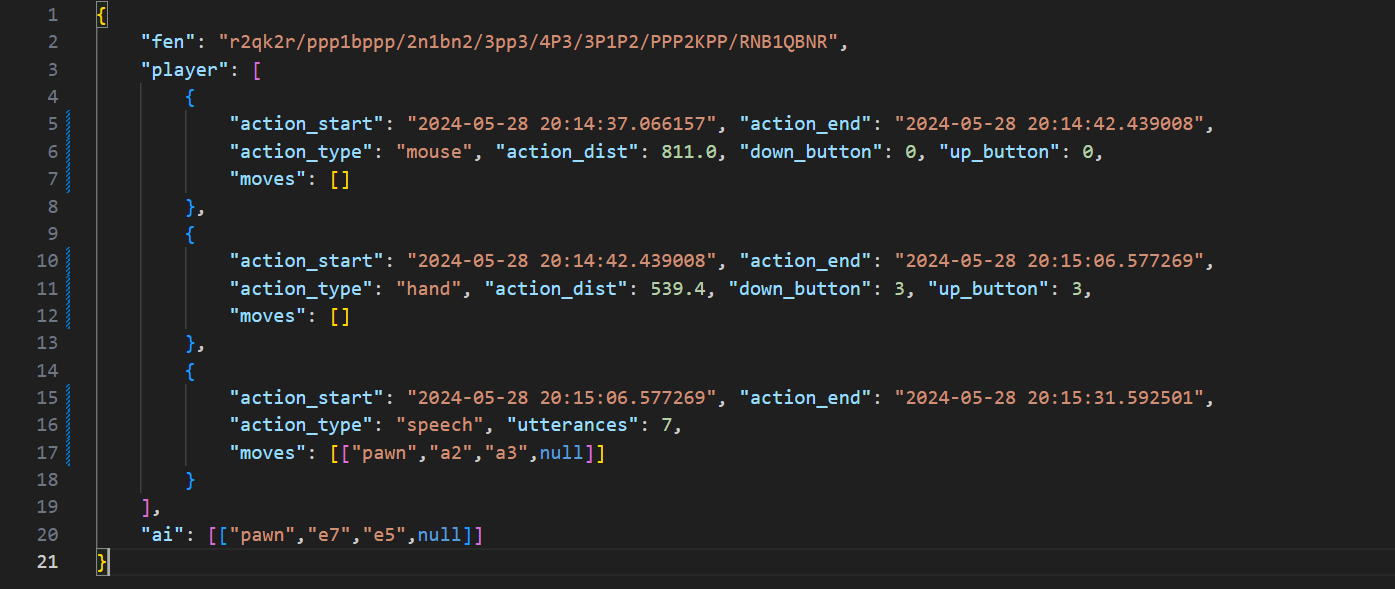
\includegraphics[width=.98\textwidth]{images/example_record3.png}
    \end{figure}
    Each recording is organized into two primary sections, namely \textbf{Player Actions} and \textbf{AI Moves}.
\end{frame}

\begin{frame}{Recording System II}
    
    Each action performed contains information about :   
    \begin{itemize}
            \item \texttt{Type} : Mouse, Hand or Voice
            \item \texttt{Start \& End Time} : Time of Action Start and End 
            \item \texttt{Moves} :  (Source Piece, Source Square, Target Piece, Target Square, Promotion Piece)
            \item \texttt{Optional} : Utterances, Hand \& Mouse Distance, Hand \& Mouse Bottons Up and Down 
    \end{itemize}
\end{frame}


\begin{frame}{Results, Total Time}
    \begin{figure}
        \centering
        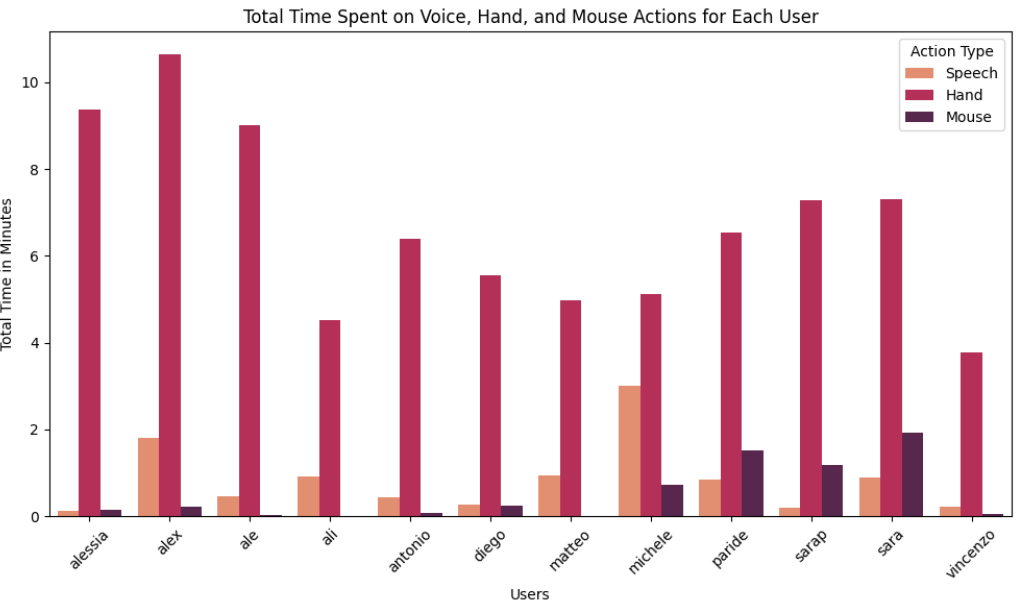
\includegraphics[width=.8\textwidth]{images/total_time.png}
        \caption{\textbf{Total Time} (seconds) on Voice, Hand and Mouse Actions per user}
    \end{figure}
\end{frame}

\begin{frame}{Results, APM}
    \begin{figure}
        \centering
        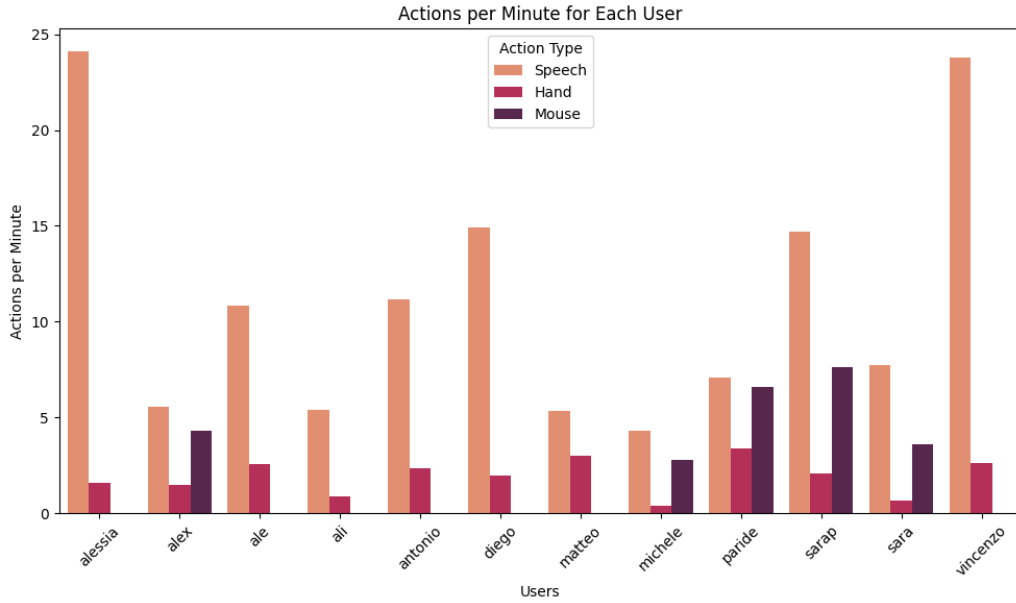
\includegraphics[width=.8\textwidth]{images/actions_per_minutes.png}
        \caption{\textbf{Actions per Minute} per user}
    \end{figure}
\end{frame}

\begin{frame}{Results, Total Actions}
    \begin{figure}
        \centering
        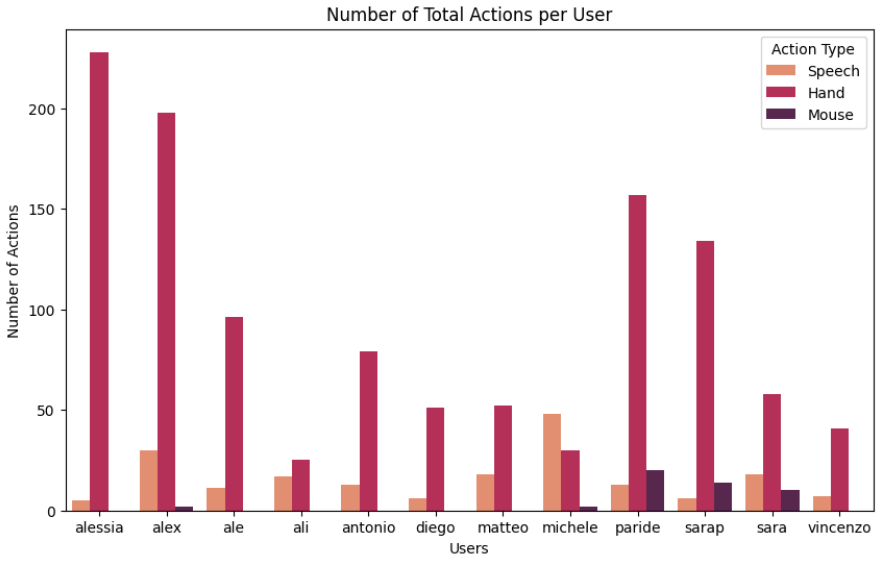
\includegraphics[width=.8\textwidth]{images/total_actions.png}
        \caption{Number of \textbf{Total} Actions per user}
    \end{figure}
\end{frame}

\begin{frame}{Results, Legal Actions}
    \begin{figure}
        \centering
        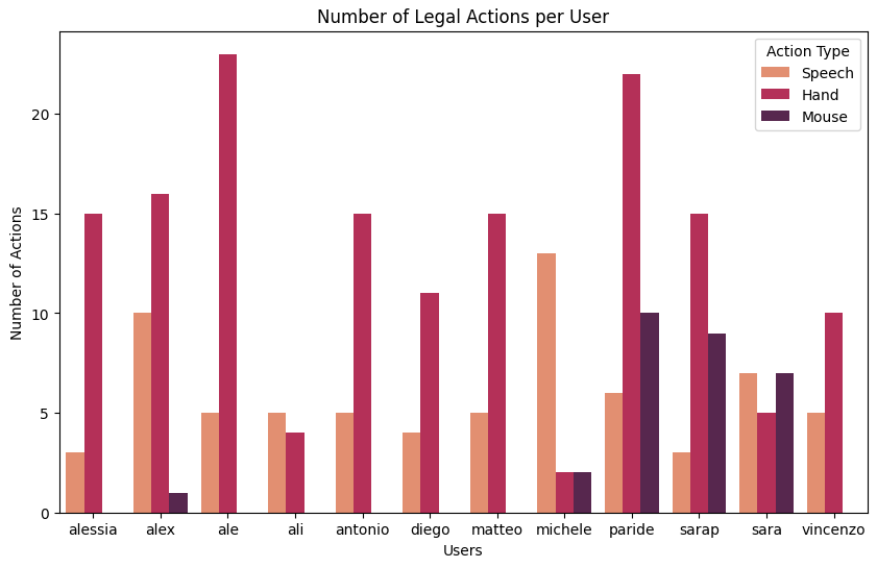
\includegraphics[width=.8\textwidth]{images/legal_actions.png}
        \caption{Number of \textbf{Legal} Actions per user}
    \end{figure}
\end{frame}

\begin{frame}{Results, Error rate hand}
    \begin{figure}
        \centering
        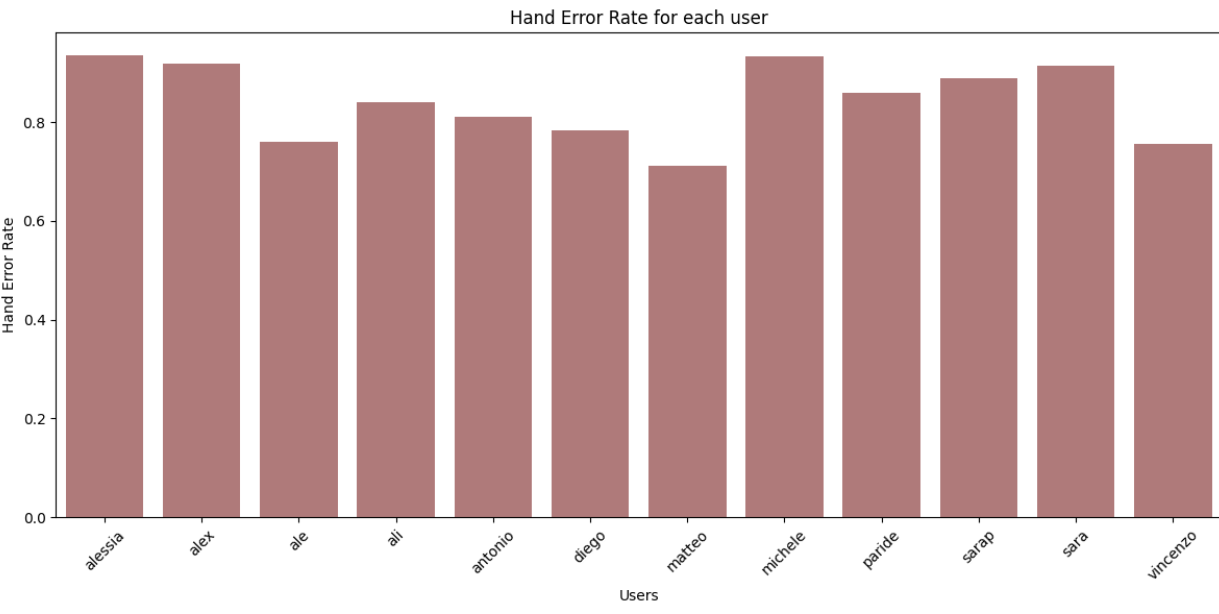
\includegraphics[width=.8\textwidth]{images/hand_error_rate.png}
        \caption{\textbf{Error rate} for \textbf{Hand} actions}
    \end{figure}
\end{frame}

\begin{frame}{Results, Error rate voice}
    \begin{figure}
        \centering
        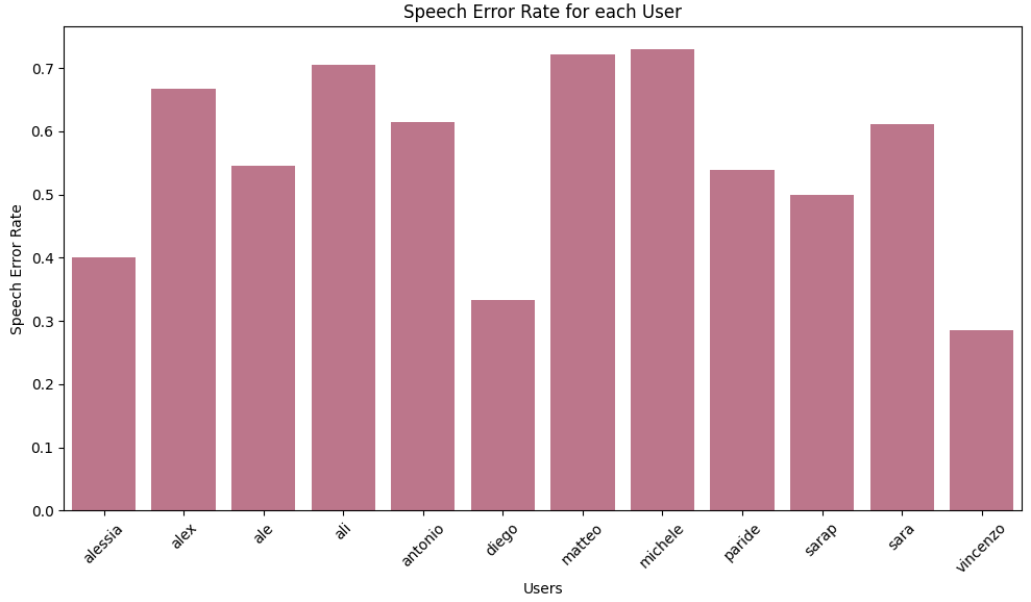
\includegraphics[width=.8\textwidth]{images/speech_error_rate.png}
        \caption{\textbf{Error rate} for \textbf{Voice} actions}
    \end{figure}
\end{frame}

\begin{frame}{Conclusions}
    Something something
    \begin{figure}
        \centering
        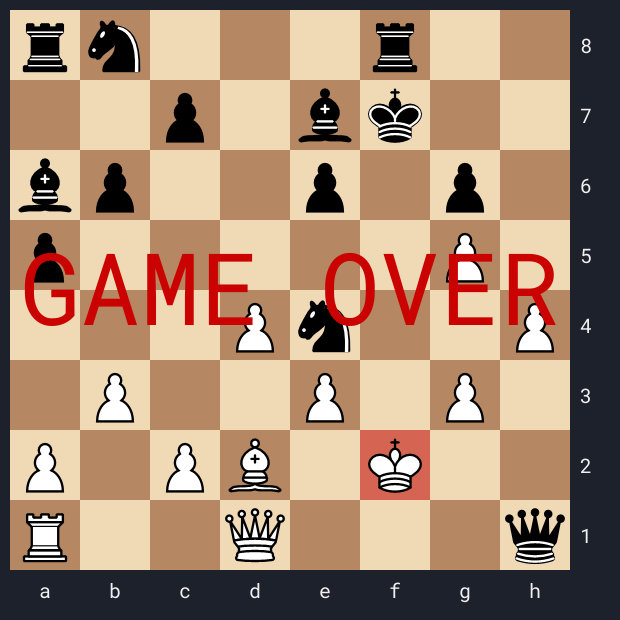
\includegraphics[width=.45\textwidth]{images/game_over_small.png}
        \caption{Fin.}
    \end{figure}
\end{frame}

\end{document}